\documentclass[12pt]{article}
\newif\ifanswer\answertrue%\answerfalse% comment out to show/hide answers
\usepackage{../preamble3}% preamble always after \newif\ifanswer
%\pagenumbering{gobble}
\title{Art Of Problem Solving - AMC 10 \\ Week 10}
\author{Patrick \& James Toche}
\date{August 14, 2021}

\begin{document}
\maketitle
\begin{minipage}{\textwidth}
\begin{abstract}\setlength{\parindent}{0pt}%
Notes on the AMC-10 Course by Art Of Problem Solving (AOPS).
Copyright restrictions may apply. Written for personal use. 
Please report typos and errors over at \url{https://github.com/ptoche/Math/tree/master/aops}. 
\end{abstract}
\end{minipage}

\thispagestyle{empty}
\clearpage


%%%%%%%%%%%%%%%%%%%%%%%%%%%%%%%%%%%%%%%%%%%%%%%%%%%%%%%%%%%%%%%%%%%%%%%%
\subsection*{1.}

\nopagebreak

Two fair coins are to be tossed once. For each head that results, one fair die is to be rolled. What is the probability that the sum of the die rolls is odd? (Note that if no die is rolled, the sum is 0.)

\nopagebreak

\fbox{(A) $\dfrac{3}{8}$ \quad (B) $\dfrac{1}{2}$ \quad (C) $\dfrac{43}{72}$ \quad (D) $\dfrac{5}{8}$ \quad (E) $\dfrac{2}{3}$}

\begin{answer}
A fair die has $6$ faces with three odd values and three even values: The probability that a single roll yields an odd value is therefore one-half. 
Two fair dice rolled together have six odd values and six even values, with sums also distributed equally between odd and even. 
Indeed 
\begin{align*}
\text{with probability} \quad \frac{1}{2}: \quad
& 
\begin{cases}
\quad   \text{odd} + \text{odd} & = \quad \text{even} \\
\quad \text{even} + \text{even} & = \quad \text{even} \\
\end{cases} \\
\text{with probability} \quad \frac{1}{2}: \quad
& 
\begin{cases}
\quad  \text{odd} + \text{even} & = \quad \text{odd} \\
\quad  \text{even} + \text{odd} & = \quad \text{odd} \\
\end{cases}
\end{align*}
and can also be verified by enumerating and counting the cases: 
\begin{center}
\renewcommand\arraystretch{1}
\begin{tabular}{*{7}{c}}
\toprule
  &            1 &           2 &           3 &           4 &           5 &           6\\
\midrule
1 & \text{even} &  \text{odd} & \text{even} &  \text{odd} & \text{even} &  \text{odd}\\
2 &  \text{odd} & \text{even} &  \text{odd} & \text{even} & \text{odd} & \text{even}\\
3 & \text{even} &  \text{odd} & \text{even} &  \text{odd} & \text{even} &  \text{odd}\\
4 &  \text{odd} & \text{even} &  \text{odd} & \text{even} &  \text{odd} & \text{even}\\
5 & \text{even} &  \text{odd} & \text{even} &  \text{odd} & \text{even} &  \text{odd}\\
6 &  \text{odd} & \text{even} &  \text{odd} & \text{even} &  \text{odd} & \text{even}\\
\bottomrule
\end{tabular}
\end{center}

Let H denote Heads and T denote Tails.
The coin tosses have four possible outcomes HH, TT, HT, TH. The probability of each of these cases is one in four. The mixed cases HT and TH have the same implication, so they can be combined. 

\subsubsection*{TT}
Occurs with probability $\dfrac{1}{4}$. No die is rolled. The sum associated with this case is odd with probability $0$ (since $0$ is an even number).

\subsubsection*{HT \& TH}
Occurs with probability $\dfrac{1}{2}$. Only one die is rolled. The sum associated with this case is odd with probability $\dfrac{1}{2}$.

\subsubsection*{HH}
Occurs with probability $\dfrac{1}{4}$. Two dice are rolled. The sum associated with this case is odd with probability $\dfrac{1}{2}$ (see above).

Putting it all together, the probability that the sum of the rolls is odd is
\begin{align*}
& \frac{1}{4} \cdot 0 + \frac{1}{2} \cdot \frac{1}{2} + \frac{1}{4} \cdot \frac{1}{2} \\[1ex]
  & = \frac{1}{4} + \frac{1}{8} 
    = \frac{3}{8}
\end{align*}
\begin{empheq}[box={\mathbox[colback=white]}]{equation*}
    \text{probability}~ = \frac{3}{8}
\end{empheq} 
\end{answer}
%%%%%%%%%%%%%%%%%%%%%%%%%%%%%%%%%%%%%%%%%%%%%%%%%%%%%%%%%%%%%%%%%%%%%%%%

\iftoggle{showAnswers}{\newpage}

%%%%%%%%%%%%%%%%%%%%%%%%%%%%%%%%%%%%%%%%%%%%%%%%%%%%%%%%%%%%%%%%%%%%%%%%
\subsection*{2.}

\nopagebreak

A dart board is a regular octagon divided into regions as shown. Suppose that a dart thrown at the board is equally likely to land anywhere on the board. What is the probability that the dart lands within the center square?

\nopagebreak

\begin{center}
  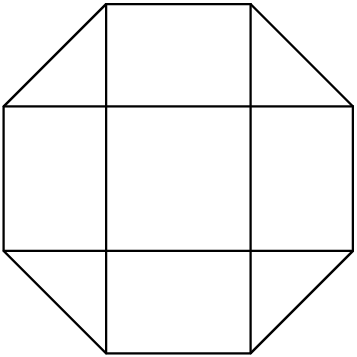
\includegraphics[height=3cm,page=1]{2021-08-14-figure-02}
\end{center}

\nopagebreak

\fbox{(A) $\dfrac{\sqrt{2}-1}{2}$ \quad (B) $\dfrac{1}{4}$ \quad (C) $\dfrac{2-\sqrt{2}}{2}$ \quad (D) $\dfrac{\sqrt{2}}{4}$ \quad (E) $2-\sqrt{2}$}

\begin{answer}
Without loss of generality, let the side lengths of the dart board and the side lengths of the center square be $\sqrt{2}$ (without loss of generality because we calculate a ratio). It follows that the side length of the legs of the triangles in the corners are equal to $1$.
\begin{align*}
\text{area of square} 
  & = \sqrt{2} \cdot \sqrt{2} = 2 \\ 
\text{area of octagon} 
  & = (\sqrt{2})^2 + 4(1 \cdot \sqrt{2}) + 4(1 \cdot 1 \cdot \frac{1}{2}) \\
  & = 2 + 4\sqrt{2} + 2 \\
  & = 4 + 4\sqrt{2}
\end{align*}
Area of the center square divided by the area of the octagon:
\begin{align*}
\frac{\text{area of square}}{\text{area of octagon}}
 & = \frac{2}{4+4\sqrt{2}} \\
 & = \frac{1}{2+2\sqrt{2}} \cdot \frac{2-2\sqrt{2}}{2-2\sqrt{2}} \\
 & = \frac{2-2\sqrt{2}}{-4} \\
 & = \frac{\sqrt{2}-1}{2}
\end{align*}
\begin{empheq}[box={\mathbox[colback=white]}]{equation*}
    \text{probability}~ = \frac{\sqrt{2}-1}{2}
\end{empheq} 
\end{answer}
%%%%%%%%%%%%%%%%%%%%%%%%%%%%%%%%%%%%%%%%%%%%%%%%%%%%%%%%%%%%%%%%%%%%%%%%

\iftoggle{showAnswers}{\newpage}

%%%%%%%%%%%%%%%%%%%%%%%%%%%%%%%%%%%%%%%%%%%%%%%%%%%%%%%%%%%%%%%%%%%%%%%%
\subsection*{3.}

\nopagebreak

Bernardo randomly picks 3 distinct numbers from the set $\{1, 2, 3, 4, 5, 6, 7, 8, 9\}$ and arranges them in descending order to form a 3-digit number. Silvia randomly picks 3 distinct numbers from the set $\{1, 2, 3, 4, 5, 6, 7, 8\}$ and also arranges them in descending order to form a 3-digit number. What is the probability that Bernardo's number is larger than Silvia's number?

\nopagebreak

\fbox{(A) $\dfrac{47}{72}$ \quad (B) $\dfrac{37}{56}$ \quad (C) $\dfrac{2}{3}$ \quad (D) $\dfrac{49}{72}$ \quad (E) $\dfrac{39}{56}$}

\begin{answer}
\subsubsection*{Case 1: Bernardo picks $\mathrm{9}$}
Bernardo picks a $9$ with probability $\dfrac{1}{3}$, since randomly selecting $3$ digits from $9$ will contain the $9$ in one out of three cases. A more general approach is to count. There is only one way to select a $9$, there are $\displaystyle\binom{8}{2}$ ways to select the other two digits, and altogether there are $\displaystyle\binom{9}{3}$ ways to select any three digits from the available nine. Thus,
\begin{align*}
\frac{1 \cdot \displaystyle\binom{8}{2}}{\displaystyle\binom{9}{3}} 
  = \frac{\dfrac{8\cdot7}{2}}{\dfrac{9\cdot8\cdot7}{3\cdot2\cdot1}}
  = \frac{1}{3}
\end{align*}
and, conditioning on picking the $9$, Bernardo wins with probability $1$. 

\subsubsection*{Case 2: Bernardo does not pick $\mathrm{9}$}
Bernardo does not pick $9$ with probability equal to the complement probability, that is
\begin{align*}
1- \frac{1}{3} 
  = \frac{2}{3}
\end{align*}
and, conditioning on that selection, wins with probability equal to that of Silvia's. Isn't that just one-half ? Not quite! If they both pick the same digits, the game is a tie. What is the probability of a tie? It is equal to the probability that Bernardo and Silvia both pick the same three digits from the available $8$ digits $\{1,2,3,4,5,6,7,8\}$. Given Bernardo's three digits, whatever they may be, the probability that Silvia picks the same three digits is one divided by the number of ways to pick any three digits from the available eight, or
\begin{align*}
\frac{1}{\displaystyle\binom{8}{3}}
  = \frac{(8-3)!\,3!}{8!}
  = \frac{3\cdot2}{8\cdot7\cdot6} 
  = \frac{1}{56}
\end{align*}
The probability that Bernardo's number is larger than Silvia's is therefore
\begin{align*}
\frac{1}{2}\cdot \left(1-\dfrac{1}{56}\right)
  = \frac{55}{112}
\end{align*}
(that is also the probability that Silvia's number is larger than Bernardo's).

\subsubsection*{Case 1 and 2 Together}
Considering both cases together: 
\begin{align*}
  & \frac{1}{3} \cdot 1 + \frac{2}{3} \cdot \frac{55}{112} \\[1ex]
  & = \frac{1}{3} + \frac{55}{168} \\[1ex]
  & = \frac{56 + 55}{168} \\[1ex]
  & = \frac{111}{168}
    = \frac{37}{56} 
    \approx 0.66
\end{align*}
\begin{empheq}[box={\mathbox[colback=white]}]{equation*}
    \text{probability}~ = \frac{37}{56}
\end{empheq} 
\end{answer}
%%%%%%%%%%%%%%%%%%%%%%%%%%%%%%%%%%%%%%%%%%%%%%%%%%%%%%%%%%%%%%%%%%%%%%%%

\iftoggle{showAnswers}{\newpage}

%%%%%%%%%%%%%%%%%%%%%%%%%%%%%%%%%%%%%%%%%%%%%%%%%%%%%%%%%%%%%%%%%%%%%%%%
\subsection*{4.}

\nopagebreak

Positive integers $a$, $b$, and $c$ are randomly and independently selected with replacement from the set $\{1, 2, 3, \dots, 2010\}$. What is the probability that $abc+ab+a$ is divisible by 3?

\nopagebreak

\fbox{(A) $\dfrac{1}{3}$ \quad (B) $\dfrac{29}{81}$ \quad (C) $\dfrac{31}{81}$ \quad (D) $\dfrac{11}{27}$ \quad (E) $\dfrac{13}{27}$}

\begin{answer}
An integer $n$ is divisible by $3$, denoted $3\mid{n}$ ($n$ divides into $3$), if it has a zero residue (aka remainder); that is the $(k,r)$ pair such that $n=3k+r$ has $r=0$; otherwise, if $r=1$ or $r=2$, then $n$ is not divisible by $3$. Note that if $r=1$, $n$ must be even.

Let $n=abc+ab+a$. Since $n=a(bc+b+1)$, it follows that $3\mid{a}$ implies $3\mid{n}$ (that is, if $a$ is divisible by $3$, then so is $n$). And since $3\mid{2010}$, this occurs with probability exactly $1/3$. 

Next, turn to the case where $a$ is not divisible by $3$. If $3\nmid{a}$, then $3\mid{n}$ only if $3\mid{(bc+b+1)}$. To state this in terms of modulo arithmetic and residues, only if $b(c+1)\equiv2$ modulo $3$, which can be split into two cases:
\begin{align*}
  b \equiv 1 \pmod{3} &, \quad c \equiv 1 \pmod{3} \implies b(c+1) \equiv 2 \pmod{3}\\
 b \equiv 2 \pmod {3} &, \quad c \equiv 0 \pmod{3} \implies b(c+1) \equiv 2 \pmod{3}
\end{align*}
Since the integers are randomly and independently selected with replacement, any one of the three residue classes is equiprobable, e.g. $b \equiv 1$ with probability $1/3$. Thus, each of the two cases above occurs with probability $(1/3)\times(1/3)$.
Putting it all together,
\begin{align*}
  & \dfrac{1}{3} + \dfrac{2}{3} \left( \dfrac{1}{3} \cdot \frac{1}{3} + \dfrac{1}{3} \cdot \frac{1}{3} \right) \\[1ex]
  & = \frac{1}{3} + \frac{4}{27} \\[1ex]
  & = \frac{13}{27}
\end{align*} 
\begin{empheq}[box={\mathbox[colback=white]}]{equation*}
    \text{probability}~ = \frac{13}{27}
\end{empheq} 
\end{answer}
%%%%%%%%%%%%%%%%%%%%%%%%%%%%%%%%%%%%%%%%%%%%%%%%%%%%%%%%%%%%%%%%%%%%%%%%

\iftoggle{showAnswers}{\newpage}

%%%%%%%%%%%%%%%%%%%%%%%%%%%%%%%%%%%%%%%%%%%%%%%%%%%%%%%%%%%%%%%%%%%%%%%%
\subsection*{5.}

\nopagebreak

Two points on the circumference of a circle of radius $r$ are selected independently and at random. From each point a chord of length $r$ is drawn in a clockwise direction. What is the probability that the two chords intersect?

\nopagebreak

\fbox{(A) $\dfrac{1}{6}$ \quad (B) $\dfrac{1}{5}$ \quad (C) $\dfrac{1}{4}$ \quad (D) $\dfrac{1}{3}$ \quad (E) $\dfrac{1}{2}$}

\begin{answer}
Points $A$ and $B$ are selected at random and a chord of length $r$ is draw clockwise. If the distance between $A$ and $B$ is smaller than $r$, the chords intersect (as with the middle figure). 
\begin{center}
  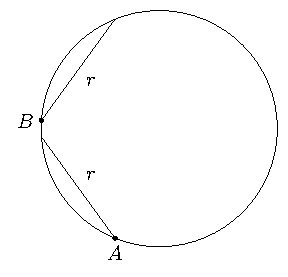
\includegraphics[height=4.5cm,page=1]{2021-08-14-figure-05}
  \hspace{20pt}
  \includegraphics[height=4.5cm,page=2]{2021-08-14-figure-05}
  \hspace{20pt}
  \includegraphics[height=4.5cm,page=3]{2021-08-14-figure-05}
\end{center}
\bigskip
The third figure shows the limit case where the chords connect at a single point. By construction, triangles $\triangle OAB$ and $\triangle OCB$ are isosceles triangle, and $\angle ABO$ and $\angle CBO$ therefore measure $60^{\circ}$. Thus $\angle ABC$ measures $120^{\circ}$. Thus arc $OAC$ has a span 
\begin{align*}
\sectorhat{OAC} = \dfrac{120^{\circ}}{360^{\circ}} = \dfrac{1}{3}
\end{align*}
of the circumference of the circle. 
For any two points $A$ and $B$ closer than that, there always is an intersection, which occurs in one-third of the cases. 
\begin{empheq}[box={\mathbox[colback=white]}]{equation*}
    \text{probability}~ = \frac{1}{3}
\end{empheq} 
\end{answer}
%%%%%%%%%%%%%%%%%%%%%%%%%%%%%%%%%%%%%%%%%%%%%%%%%%%%%%%%%%%%%%%%%%%%%%%%

\iftoggle{showAnswers}{\newpage}

%%%%%%%%%%%%%%%%%%%%%%%%%%%%%%%%%%%%%%%%%%%%%%%%%%%%%%%%%%%%%%%%%%%%%%%%
\subsection*{6.}

\nopagebreak

A bag contains two red beads and two green beads. You reach into the bag and pull out a bead, replacing it with a new red bead regardless of the color you pulled out. What is the probability that all beads in the bag are red after three such replacements?

\nopagebreak

\fbox{(A) $\dfrac{1}{8}$ \quad (B) $\dfrac{5}{32}$ \quad (C) $\dfrac{9}{32}$ \quad (D) $\dfrac{3}{8}$ \quad (E) $\dfrac{7}{16}$}

\begin{answer}

\subsubsection*{Case 1}
The green beads are selected first and second with probability
\begin{align*}
\frac{2}{4} \cdot \frac{1}{4} \cdot \frac{4}{4} 
  = \frac{1}{8}
\end{align*}

\subsubsection*{Case 2}
The green beads are selected second and third with probability
\begin{align*}
\frac{2}{4} \cdot \frac{2}{4} \cdot \frac{1}{4} 
  = \frac{1}{16}
\end{align*}

\subsubsection*{Case 3}
The green beads are selected first and third with probability
\begin{align*}
\frac{2}{4} \cdot \frac{3}{4} \cdot \frac{1}{4} 
  = \frac{3}{32}
\end{align*}

\subsubsection*{All Cases}
The probabilities are independent and may be added up:
\begin{align*}
\frac{1}{8} + \frac{3}{32} + \frac{1}{16} 
  = \frac{4}{32} + \frac{3}{32} + \frac{2}{32} 
  = \frac{9}{32}
\end{align*}
\begin{empheq}[box={\mathbox[colback=white]}]{equation*}
    \text{probability}~ = \frac{9}{32}
\end{empheq} 
\end{answer}
%%%%%%%%%%%%%%%%%%%%%%%%%%%%%%%%%%%%%%%%%%%%%%%%%%%%%%%%%%%%%%%%%%%%%%%%

\iftoggle{showAnswers}{\newpage}

%%%%%%%%%%%%%%%%%%%%%%%%%%%%%%%%%%%%%%%%%%%%%%%%%%%%%%%%%%%%%%%%%%%%%%%%
\subsection*{7.}

\nopagebreak

For a particular peculiar pair of dice, the probabilities of rolling 1, 2, 3, 4, 5, and 6 on each die are in the ratio $1:2:3:4:5:6$. What is the probability of rolling a total of 7 on the two dice?

\nopagebreak

\fbox{(A) $\dfrac{4}{63}$ \quad (B) $\dfrac{1}{8}$ \quad (C) $\dfrac{8}{63}$ \quad (D) $\dfrac{1}{6}$ \quad (E) $\dfrac{2}{7}$}

\begin{answer}
This is an unfair pair of dice. 
Let $p$ be the probability of rolling a $1$. The probability of rolling a $2$ is $2p$, of rolling a $3$, $3p$, and so on.
The sum of the probabilities must add up to one:
\begin{align*}
p + 2p + 3p + 4p + 5p + 6p 
    & = 1\\
\implies\quad
  p & = \frac{1}{21}
\end{align*}
Thus the probability of rolling a $k$ is $k/21$, for $k=1,2,3,4,5,6$. 

A roll of $7$ with two dice can be obtained with the following pairs:
\begin{align*} 
(1,6), \quad (2,5), \quad (3,4), \quad (4,3), \quad (5,2), \quad (6,1)
\end{align*}
Adding up the probabilities for each combination gives
\begin{align*} 
    \frac{1}{21} \cdot \frac{6}{21}
  + \frac{2}{21} \cdot \frac{5}{21}
  + \frac{3}{21} \cdot \frac{4}{21}
  + \frac{4}{21} \cdot \frac{3}{21}
  + \frac{5}{21} \cdot \frac{2}{21}
  + \frac{6}{21} \cdot \frac{1}{21}
  = \frac{8}{63}
\end{align*}
\begin{empheq}[box={\mathbox[colback=white]}]{equation*}
    \text{probability}~ = \frac{8}{63}
\end{empheq} 
\end{answer}
%%%%%%%%%%%%%%%%%%%%%%%%%%%%%%%%%%%%%%%%%%%%%%%%%%%%%%%%%%%%%%%%%%%%%%%%

\iftoggle{showAnswers}{\newpage}

%%%%%%%%%%%%%%%%%%%%%%%%%%%%%%%%%%%%%%%%%%%%%%%%%%%%%%%%%%%%%%%%%%%%%%%%
\subsection*{8.}

\nopagebreak

A box contains exactly five chips, three red and two white. Chips are randomly removed one at a time without replacement until all the red chips are drawn or all the white chips are drawn. What is the probability that the last chip drawn is white?

\nopagebreak

\fbox{(A) $\dfrac{3}{10}$ \quad (B) $\dfrac{2}{5}$ \quad (C) $\dfrac{1}{2}$ \quad (D) $\dfrac{3}{5}$ \quad (E) $\dfrac{7}{10}$}

\begin{answer}
There are five chips. Imagine we draw all five chips one at a time before going backwards to the end condition. If one of the white chips is drawn in fifth position, then the last chip drawn must have been red. This cannot happen if the two white chips are among the first four. This implies that the three red chips cannot have been drawn yet, giving therefore all the cases. The probability is then the number of ways to choose $2$ from $4$ divided by the total number of ways to choose $2$ from $5$:
\begin{align*}
\dfrac{\dbinom{4}{2}}{\dbinom{5}{2}} 
= \frac{\dfrac{4!}{2!(4-2)!}}{\dfrac{5!}{2!(5-2)!}}
= \frac{3}{5}
\end{align*}
\begin{empheq}[box={\mathbox[colback=white]}]{equation*}
    \text{probability}~ = \dfrac{3}{5}
\end{empheq} 
\end{answer}
%%%%%%%%%%%%%%%%%%%%%%%%%%%%%%%%%%%%%%%%%%%%%%%%%%%%%%%%%%%%%%%%%%%%%%%%

\iftoggle{showAnswers}{\newpage}

%%%%%%%%%%%%%%%%%%%%%%%%%%%%%%%%%%%%%%%%%%%%%%%%%%%%%%%%%%%%%%%%%%%%%%%%
\subsection*{9.}

\nopagebreak

Tina randomly selects two distinct numbers from the set $\{1, 2, 3, 4, 5\}$, and Sergio randomly selects a number from the set $\{1, 2, \dots, 10\}$. The probability that Sergio's number is larger than the sum of the two numbers chosen by Tina is

\nopagebreak

\fbox{(A) $\dfrac{2}{5}$ \quad (B) $\dfrac{9}{20}$ \quad (C) $\dfrac{1}{2}$ \quad (D) $\dfrac{11}{20}$ \quad (E) $\dfrac{24}{25}$}

\begin{answer}
\subsubsection*{Tina's sum is 3}
This happens in only one way, with $(1,2)$. Sergio wins if he selects any number greater than $3$. There are $7$ numbers from $4$ to $10$. Thus, $7$ ways.

\subsubsection*{Tina's sum is 4}
This happens in only one way, with $(1,3)$. Sergio wins if he selects any number greater than $4$. There are $6$ numbers from $5$ to $10$. Thus, $6$ ways.

\subsubsection*{Tina's sum is 5}
This happens in two ways, with $(1,4)$ and $(2,3)$. Sergio wins if he selects any number greater than $5$. There are $5$ numbers from $6$ to $10$. Thus, $10$ ways.

\subsubsection*{Tina's sum is 6}
This happens in two ways, with $(1,5)$ and $(2,4)$. Sergio wins if he selects any number greater than $6$. There are $4$ numbers from $7$ to $10$. Thus, $8$ ways.

\subsubsection*{Tina's sum is 7}
This happens in two ways, with $(2,5)$ and $(3,4)$. Sergio wins if he selects any number greater than $7$. There are $3$ numbers from $8$ to $10$. Thus, $6$ ways.

\subsubsection*{Tina's sum is 8}
This happens in only one way, with $(3,5)$. Sergio wins if he selects any number greater than $8$. There are $2$ numbers from $9$ to $10$. Thus, $2$ ways.

\subsubsection*{Tina's sum is 9}
This happens in only one way, with $(4,5)$. Sergio wins if he selects any number greater than $9$. There is only $1$ number. Thus, $1$ way.

\subsubsection*{Cases Combined}
Adding up the number of ways for Sergio to win gives
\begin{align*}
7 + 6 + 10 + 8 + 6 + 2 + 1 = 40
\end{align*}
The total number of ways to draw two numbers from five for Tina and one number from ten for Sergio is:
\begin{align*}
\binom{5}{2} \cdot \binom{10}{1}
  = 10 \cdot 10 
  = 100
\end{align*}
And the probability is therefore the ratio
\begin{align*}
\frac{40}{100} = \frac{2}{5}
\end{align*}
\begin{empheq}[box={\mathbox[colback=white]}]{equation*}
    \text{probability}~ = \frac{2}{5}
\end{empheq} 
\end{answer}
%%%%%%%%%%%%%%%%%%%%%%%%%%%%%%%%%%%%%%%%%%%%%%%%%%%%%%%%%%%%%%%%%%%%%%%%

\iftoggle{showAnswers}{\newpage}

%%%%%%%%%%%%%%%%%%%%%%%%%%%%%%%%%%%%%%%%%%%%%%%%%%%%%%%%%%%%%%%%%%%%%%%%
\subsection*{10.}

\nopagebreak

A bug starts at one vertex of a cube and moves along the edges of the cube according to the following rule. At each vertex the bug will choose to travel along one of the three edges emanating from that vertex. Each edge has equal probability of being chosen, and all choices are independent. What is the probability that after seven moves the bug will have visited every vertex exactly once?

\nopagebreak

\fbox{(A) $\dfrac{1}{2187}$ \quad (B) $\dfrac{1}{729}$ \quad (C) $\dfrac{2}{243}$ \quad (D) $\dfrac{1}{81}$ \quad (E) $\dfrac{5}{243}$}

\begin{answer}
The first three moves are essentially equivalent since the cube can always be rotated. Suppose the bug moves according to $A \rightarrow B \rightarrow C$.
\begin{center}
  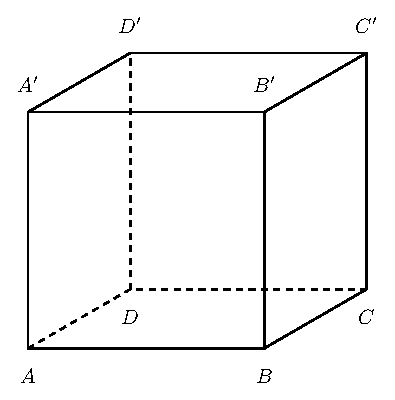
\includegraphics[height=6cm,page=1]{2021-08-14-figure-10}
\end{center}
\bigskip
At vertex $C$, the bug faces a real choice between vertex $D$ and vertex $C^{\prime}$. 

First, consider the choices available at $D$. 
At vertex $D$, only one move can take the bug along a new edge, $D\longrightarrow{D^{\prime}}$. And at vertex $D^{\prime}$, there are only two choices left to complete the course. Thus, only two paths satisfy the requirements:
\begin{align*}
A \longrightarrow B \longrightarrow C \longrightarrow D \longrightarrow D^{\prime} \longrightarrow C^{\prime} \longrightarrow B^{\prime} \longrightarrow A^{\prime}\\
A \longrightarrow B \longrightarrow C \longrightarrow D \longrightarrow D^{\prime} \longrightarrow A^{\prime} \longrightarrow B^{\prime} \longrightarrow C^{\prime}
\end{align*}

Secondly, consider the choices available at $C^{\prime}$. At vertex $C^{\prime}$, the bug faces a real choice between vertex $D^{\prime}$ and vertex $B^{\prime}$. If the bug goes to $D^{\prime}$, it then can visit either $A^{\prime}$ or $D$, but not both, so this path does not satisfy the requirements. If the bug goes to $B^{\prime}$ instead, it then goes to $A^{\prime}$ and can the complete the course in only one way:
\begin{align*}
A \longrightarrow B \longrightarrow C \longrightarrow C^{\prime} \longrightarrow B^{\prime} \longrightarrow A^{\prime} \longrightarrow D^{\prime} \longrightarrow D
\end{align*}

Only three paths satisfy the requirements starting from $A \rightarrow B \rightarrow C$. How many ways are there to choose the first three edges? At vertex $A$ the bug can go three ways, while at vertex $B$ the bug can go two ways (since going back violates the requirements). Thus, the total number of distinct paths that satisfy the requirements are:
\begin{align*}
3 \cdot 3 \cdot 2 = 18
\end{align*}
The cube has $8$ vertices and each vertex is connected to $3$ edges. However, the edge that connects back to the starting point is predetermined, so that the first and last vertices are essentially one: There are only $7$ \textit{free} vertices, and the total number of paths that go from some vertex back to it is $3^7$. The probability is therefore
\begin{align*}
\frac{3 \cdot 3 \cdot 2}{3^7}
= \frac{2}{3^5}
= \dfrac{2}{243}
\end{align*}
\begin{empheq}[box={\mathbox[colback=white]}]{equation*}
    \text{probability}~ = \frac{2}{243}
\end{empheq} 
\end{answer}
%%%%%%%%%%%%%%%%%%%%%%%%%%%%%%%%%%%%%%%%%%%%%%%%%%%%%%%%%%%%%%%%%%%%%%%%

\iftoggle{showAnswers}{\newpage}

\end{document}
